\section{Introduction}
\label{sec:introduction}

To provide an example using natbib, we use citations here~\cite{Jackson,Moore}.
In the following, the \emph{lipsum} package is exploited.

\lipsum[1-4]

\begin{figure}
    \centering
    
\includegraphics[width=0.4\columnwidth]{./figs/flatEarthEPS}
    \caption{An .eps-graphic using \emph{includegraphics}.}
    \label{fig:flatEarthEPS}
\end{figure}

\lipsum[5-6]

\begin{figure}
    \centering
    \begin{tikzpicture}
        \node at (0,0) {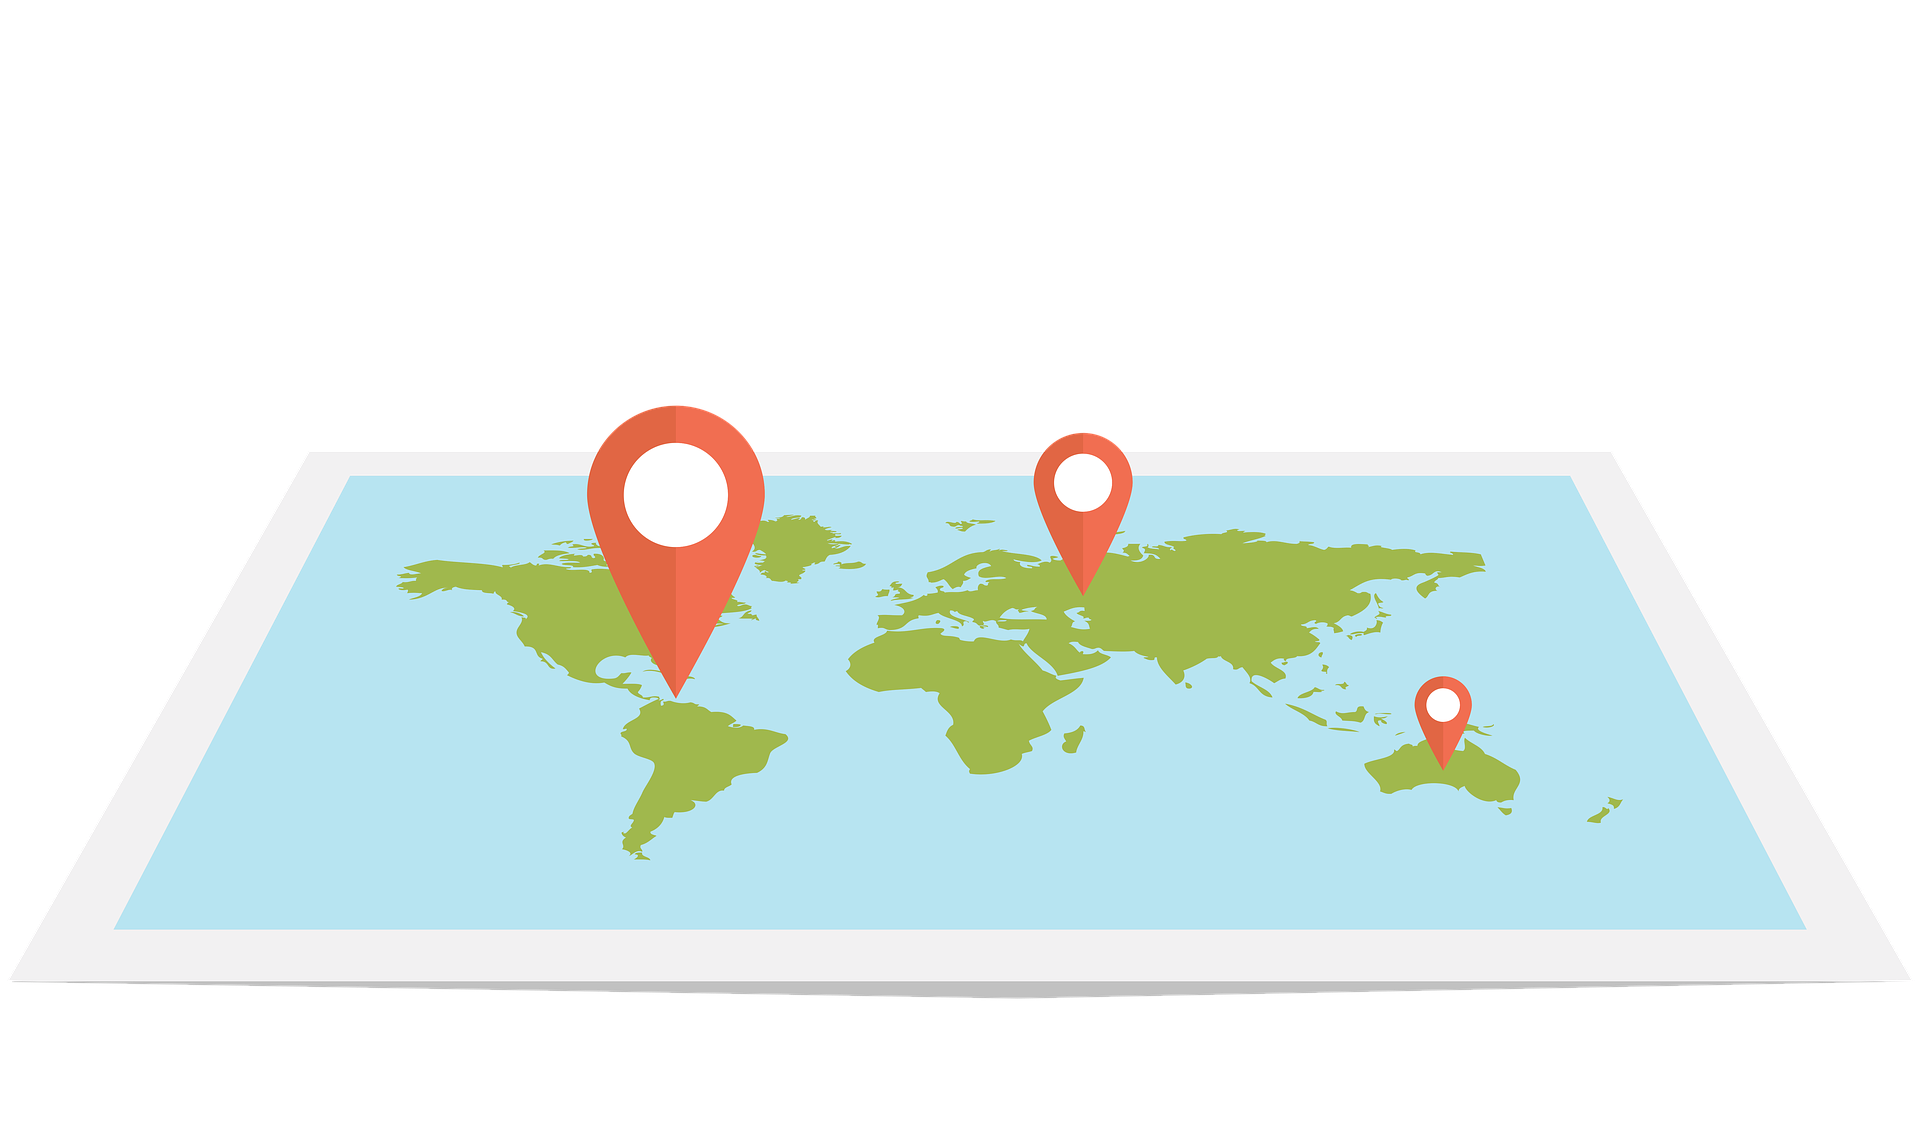
\includegraphics[width=0.6\textwidth]{./figs/flatEarthPNG}};
        \draw[->,ultra thick] (-1,1) -- (0.5,0);
    \end{tikzpicture}
    \caption{A .png-graphic using \emph{includegraphics} inside a \emph{tikz} node.}
 \label{fig:flatEarthPNGinTIKZ}
\end{figure}

\lipsum[7-10]

\begin{figure}
    \centering
    \begin{tikzpicture}
        \node at (0,0) {
\includegraphics[width=0.6\textwidth]{./figs/flatEarthEPS}};
        \draw[->,ultra thick] (-1,1) -- (0.5,0);
    \end{tikzpicture}
    \caption{An .eps-graphic using \emph{includegraphics} inside a \emph{tikz} node.}
 \label{fig:flatEarthEPSinTIKZ}
\end{figure}

\lipsum[11]

\begin{figure}
    \centering
    \includestandalone{./images/wireCrossSection}
    \caption{A simple figure representing a dashed circle.}
    \label{fig:wireCrossSection}
\end{figure}

\lipsum[12]
